\clearpage
\subsection{Studies and Updates} \label{subsec:update}

%-----------------------------------------------
\subsubsection{Weighting on generated \pt shape} \label{subsubsec:ptWeighting}
\red{TBU}

\begin{figure}[t]
    \centering
    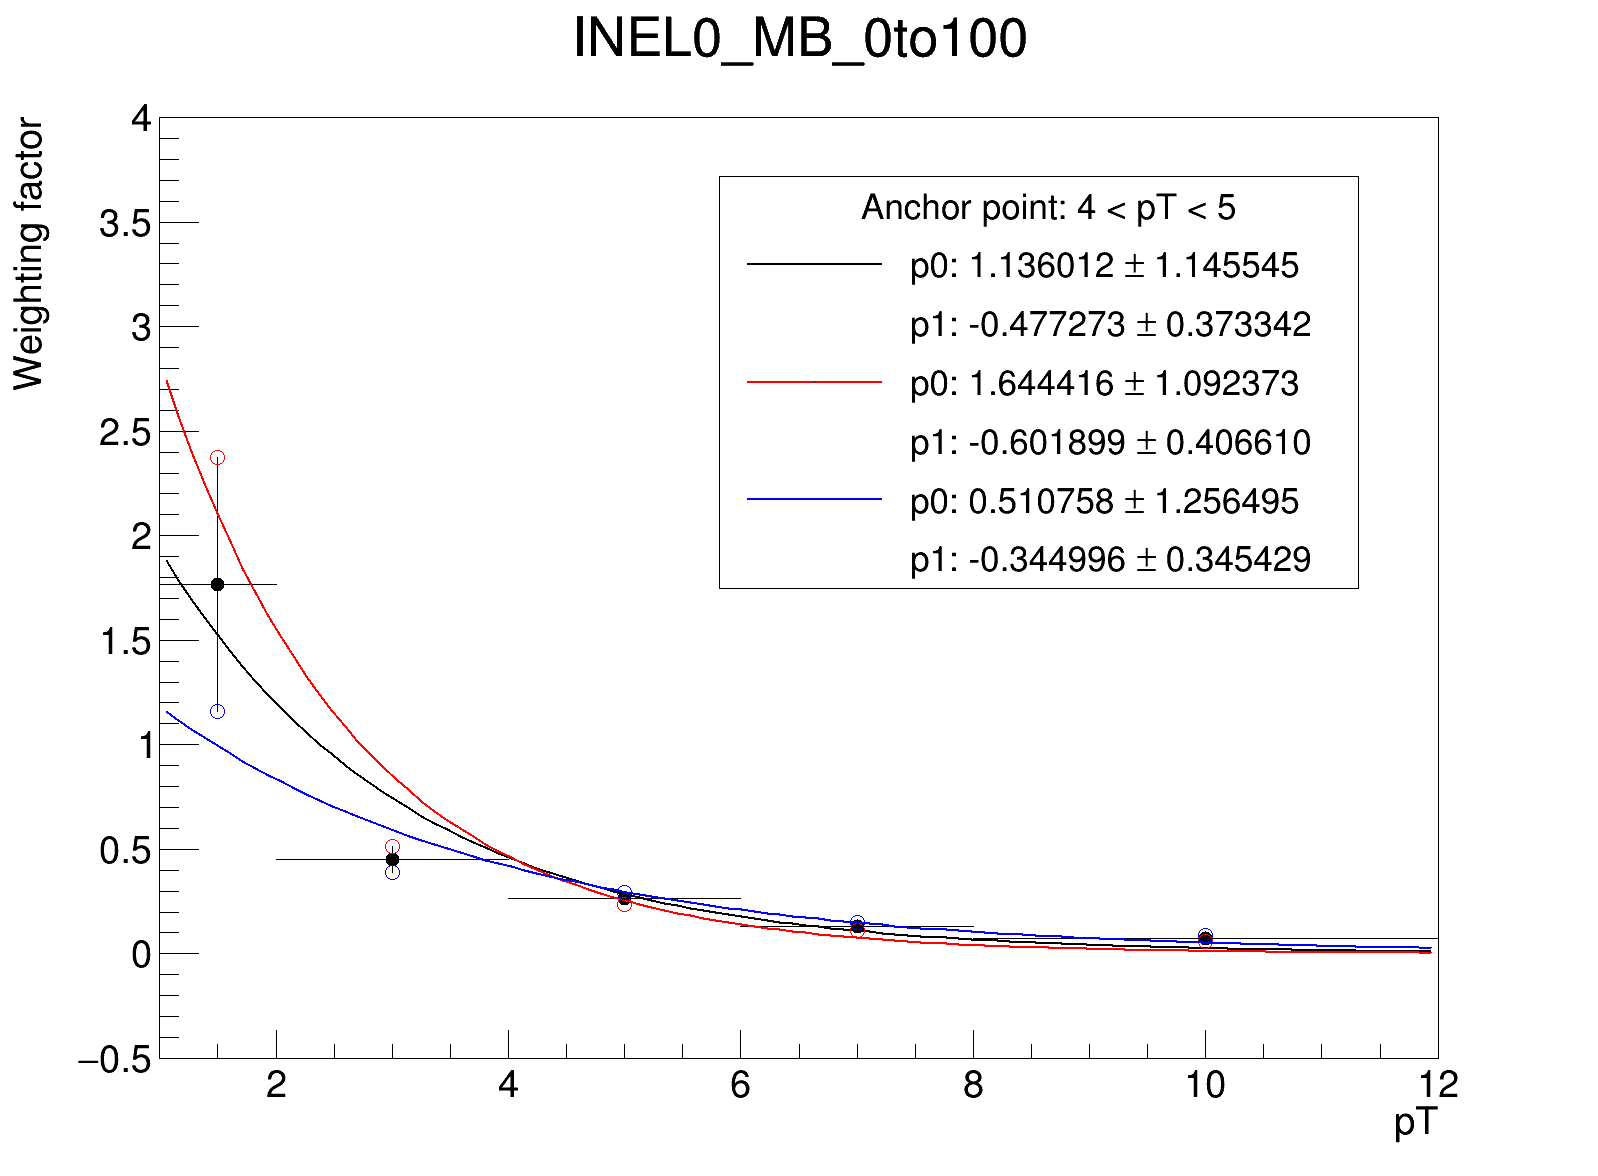
\includegraphics[width=0.45\textwidth]{plots/s2_pTW1to12_INEL0_MB_0to100.png}
    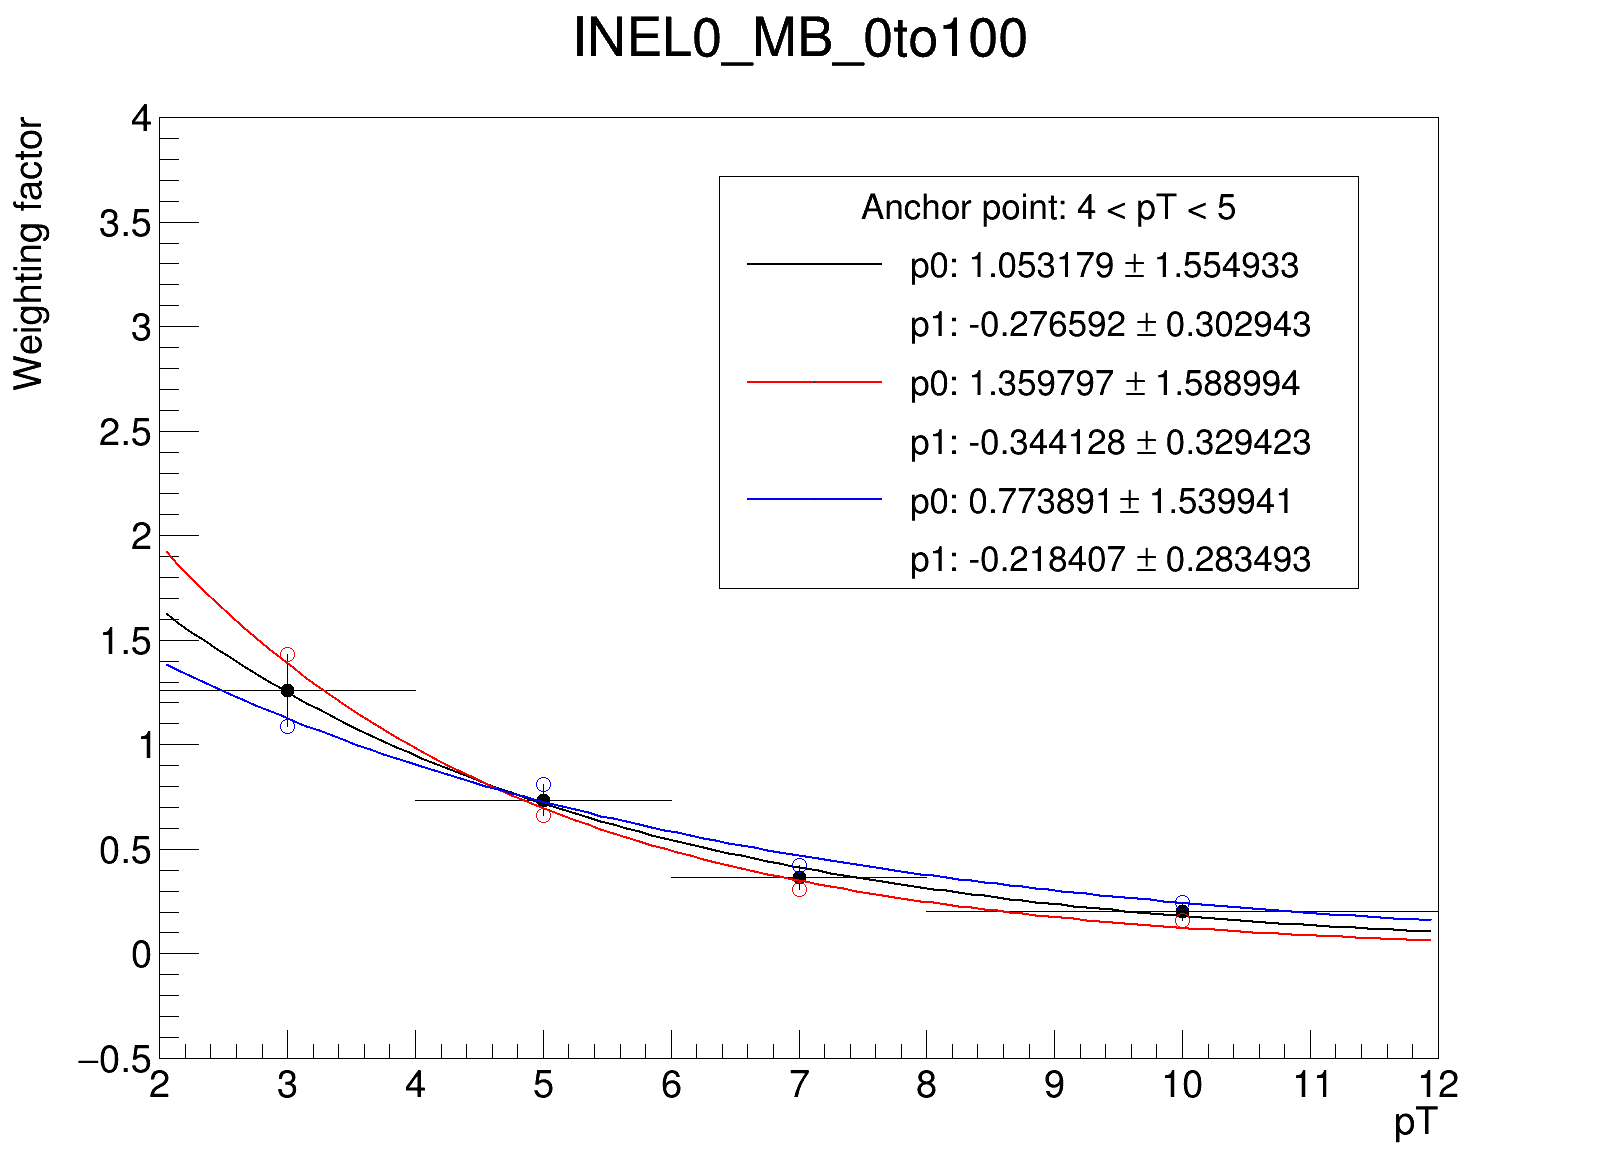
\includegraphics[width=0.45\textwidth]{plots/s2_pTW2to12_INEL0_MB_0to100.png}
    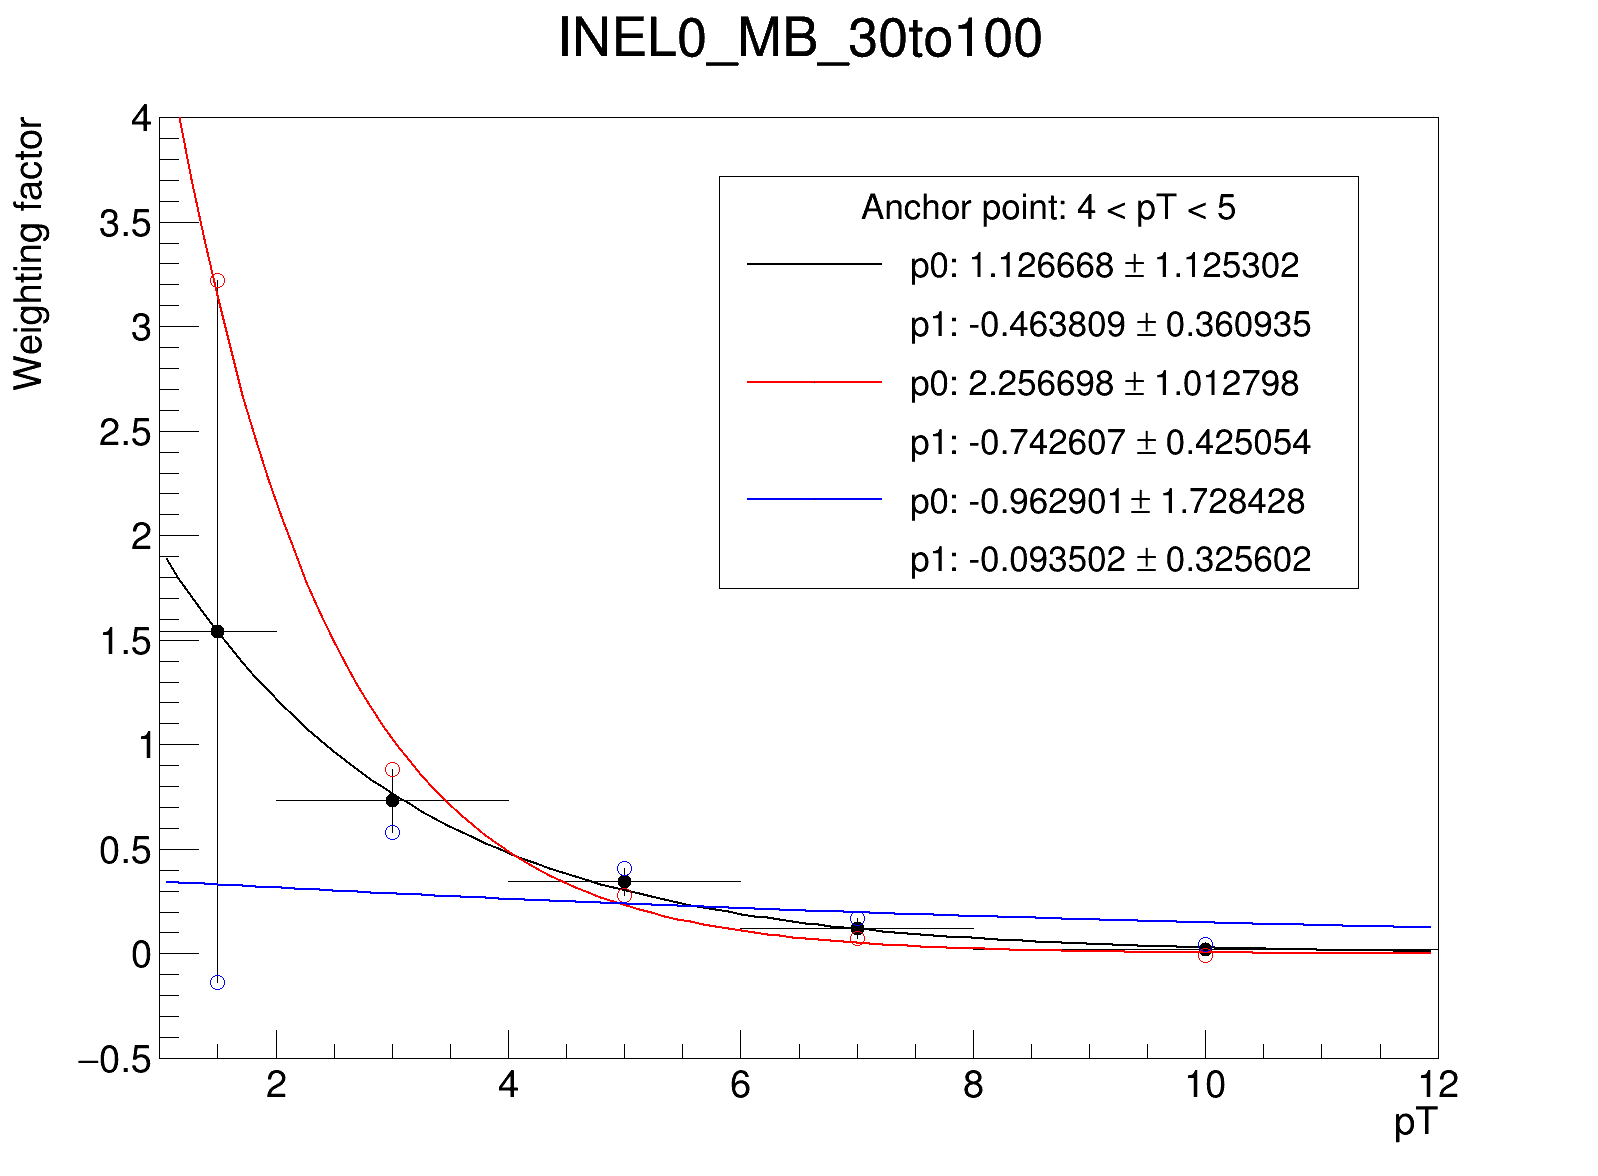
\includegraphics[width=0.45\textwidth]{plots/s2_pTW1to12_INEL0_MB_30to100.png}
    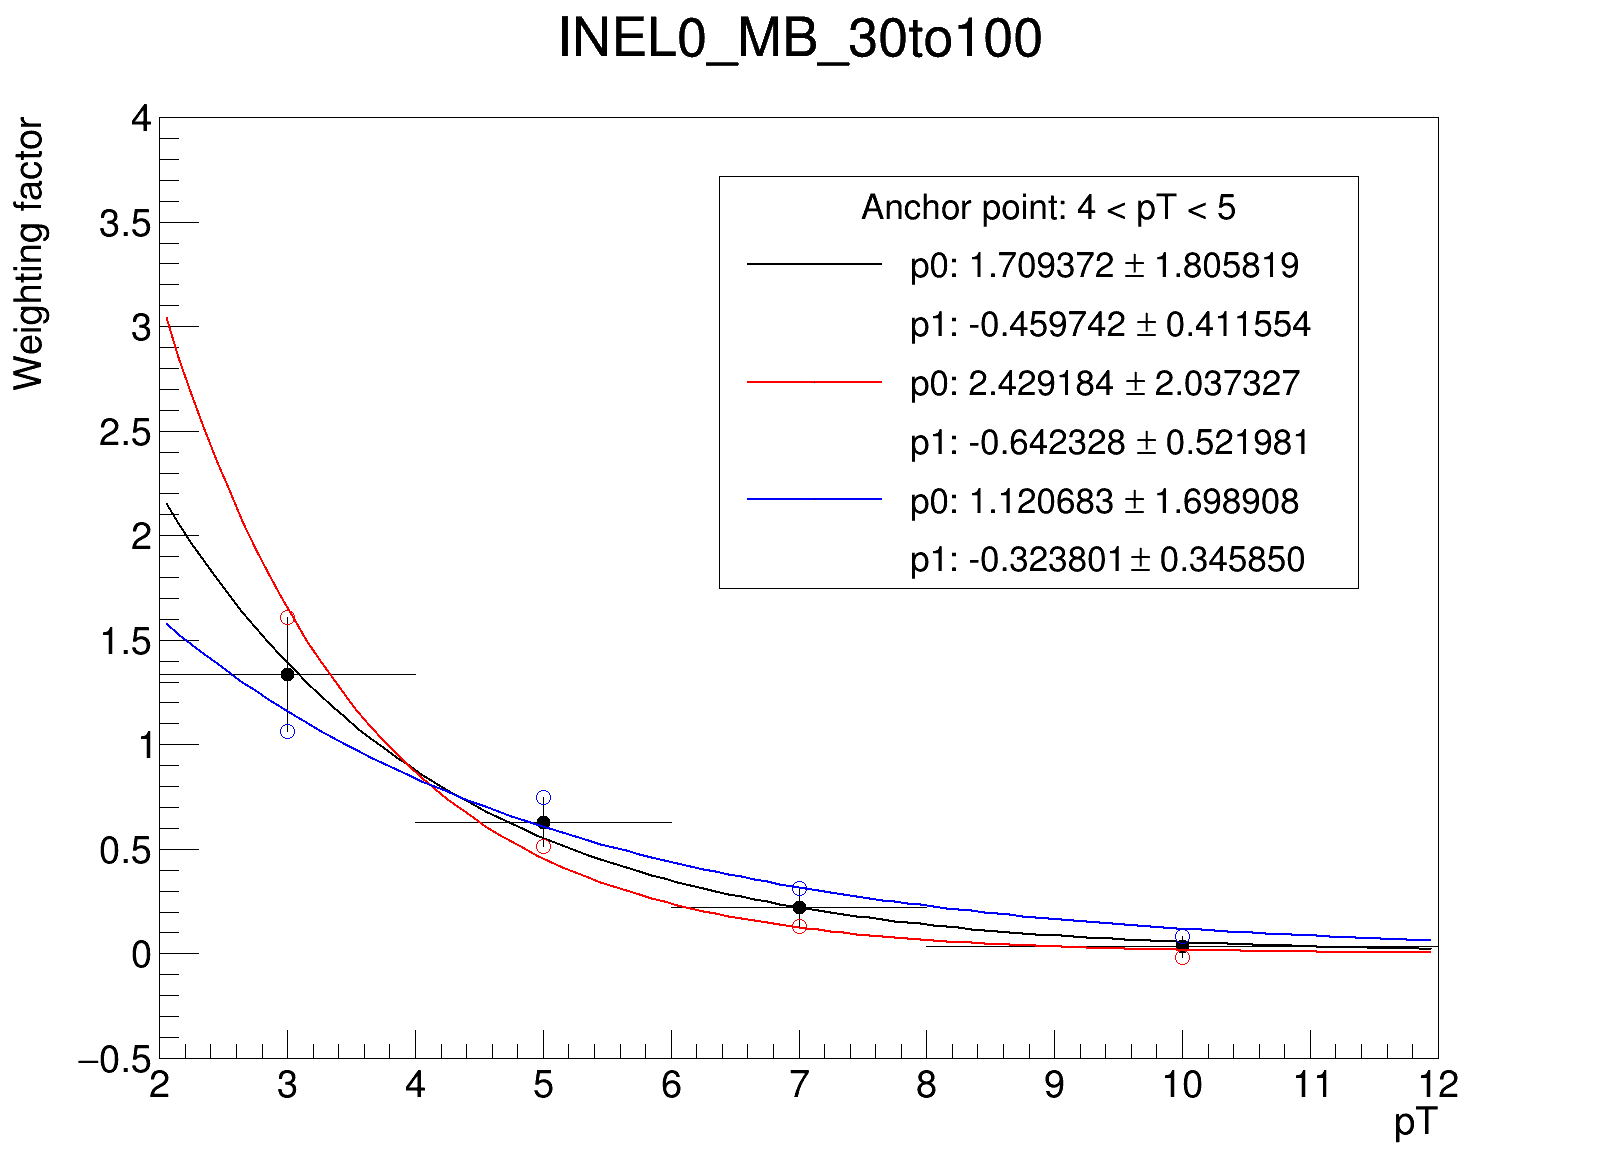
\includegraphics[width=0.45\textwidth]{plots/s2_pTW2to12_INEL0_MB_30to100.png}
    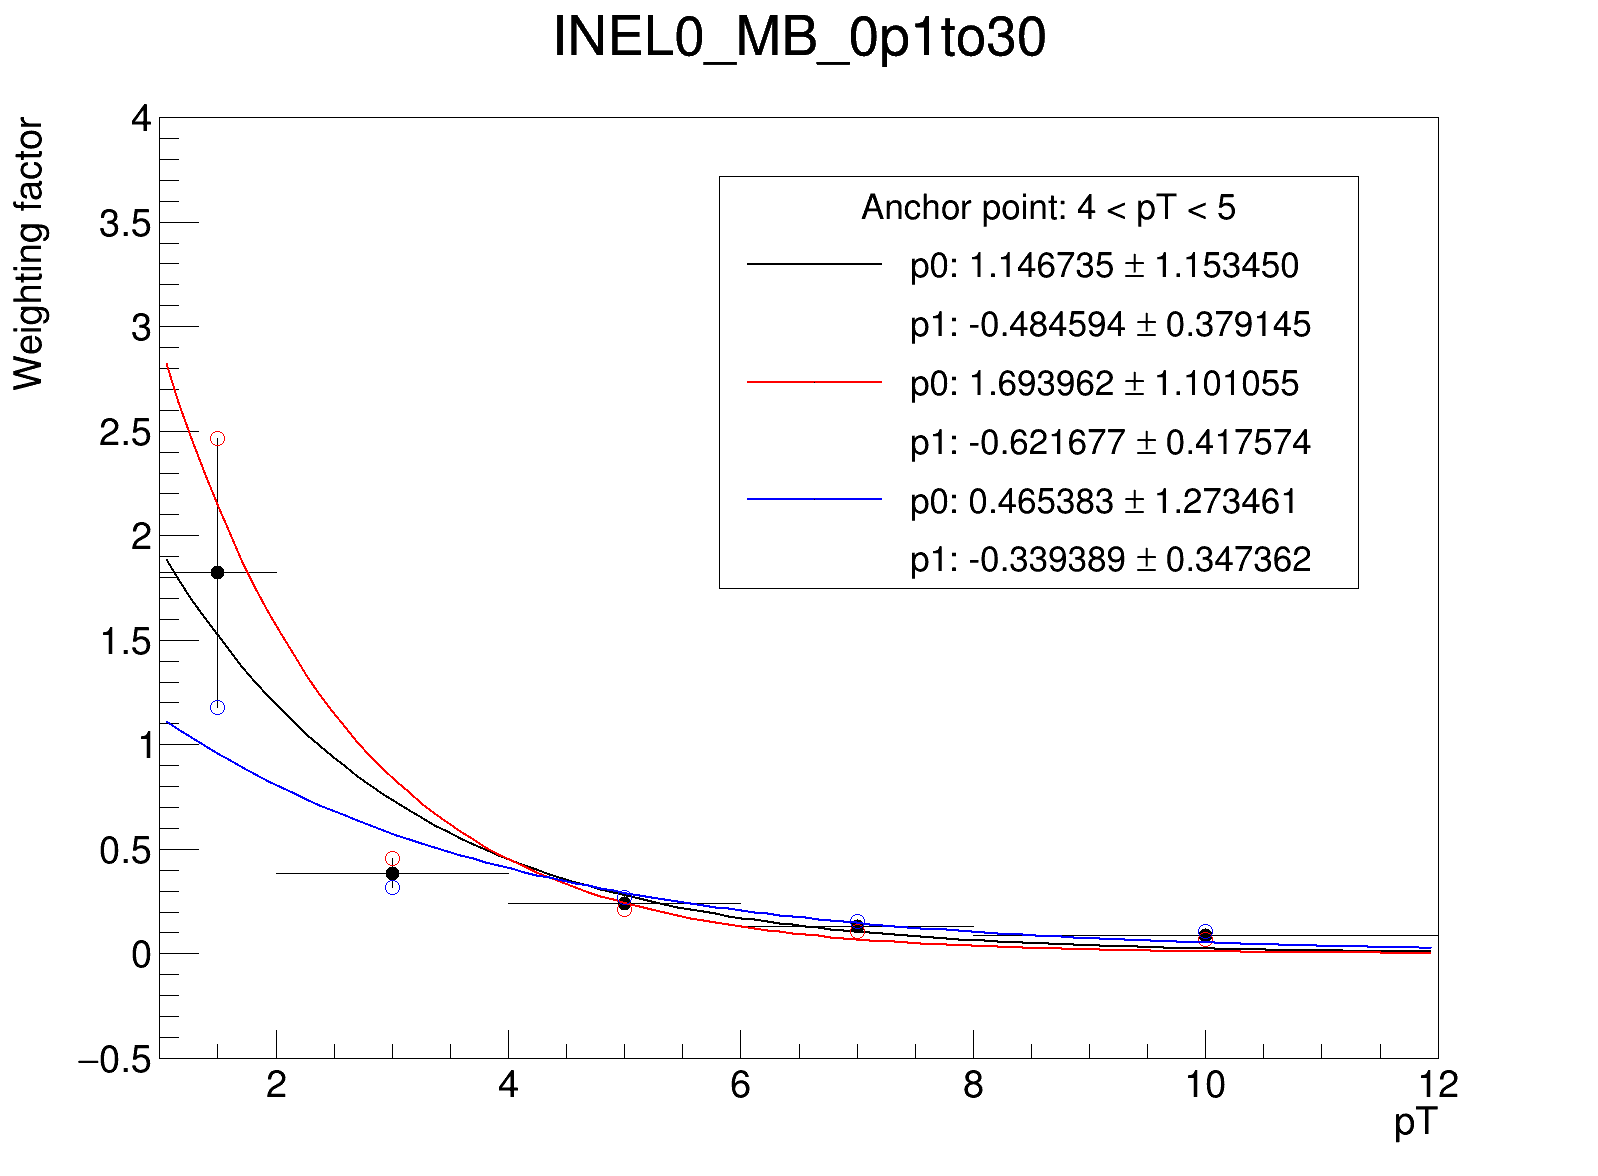
\includegraphics[width=0.45\textwidth]{plots/s2_pTW1to12_INEL0_MB_0p1to30.png}
    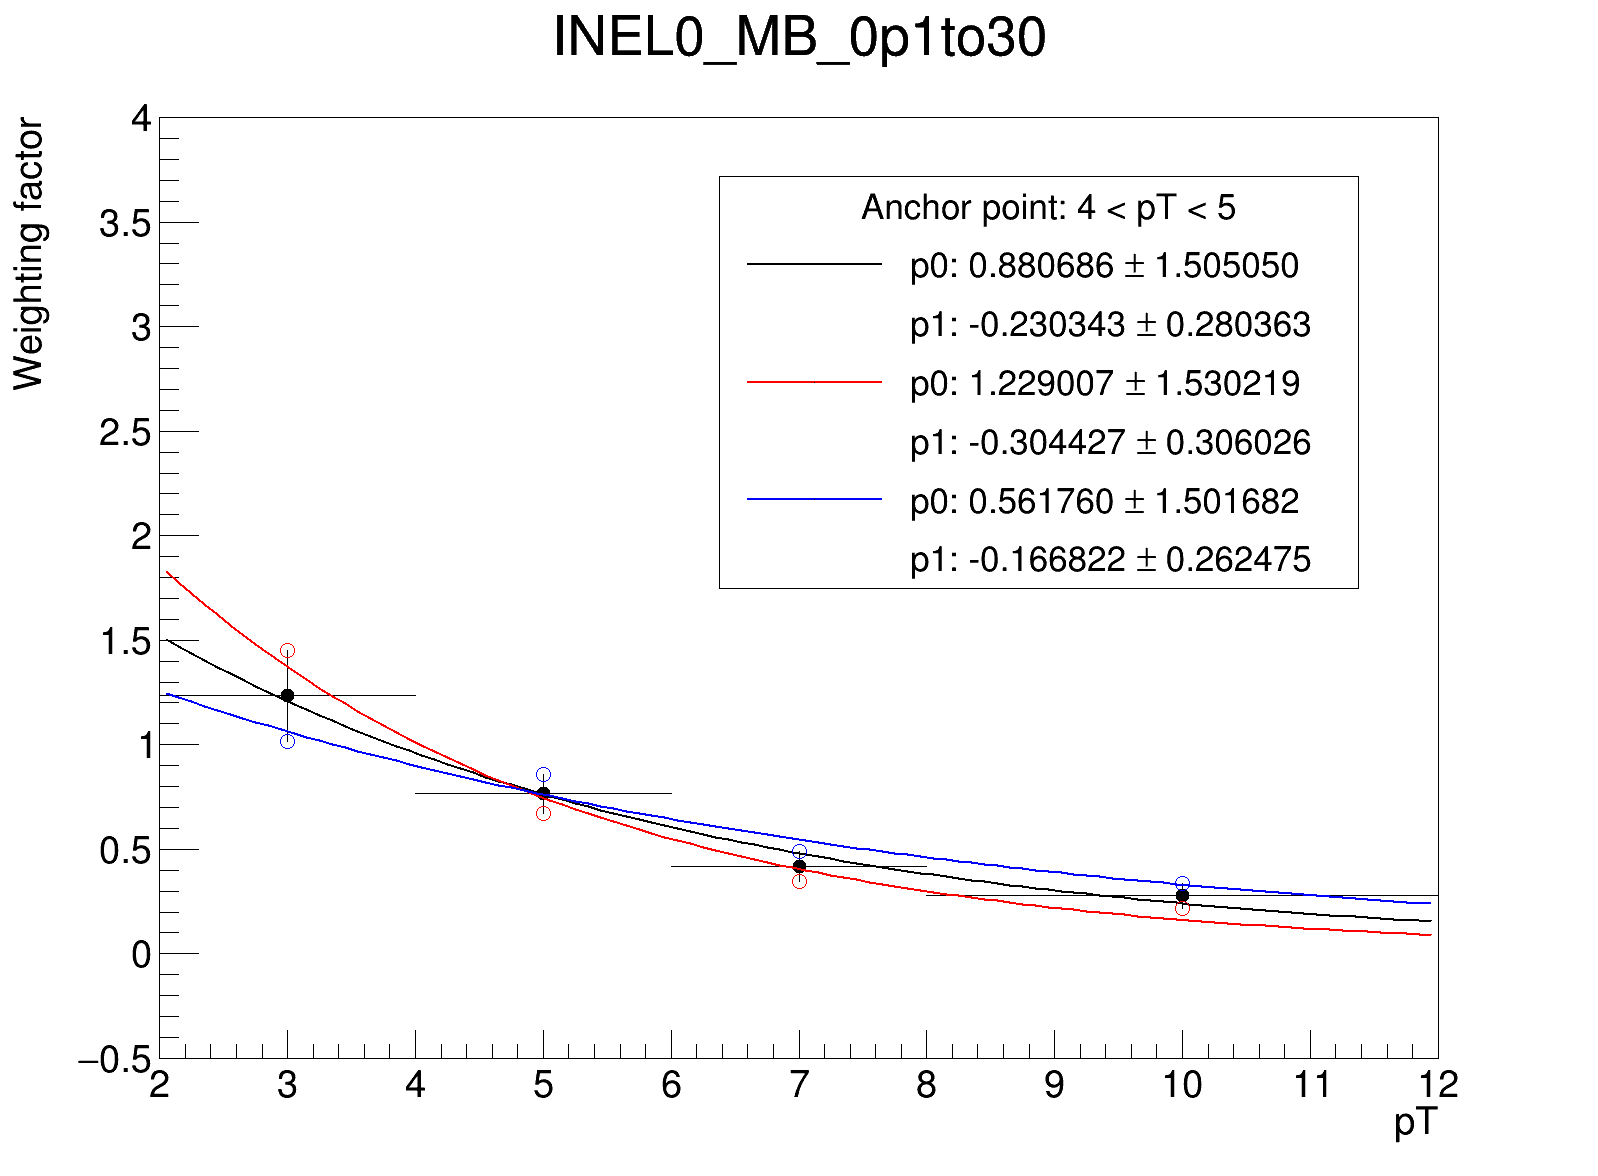
\includegraphics[width=0.45\textwidth]{plots/s2_pTW2to12_INEL0_MB_0p1to30.png}
    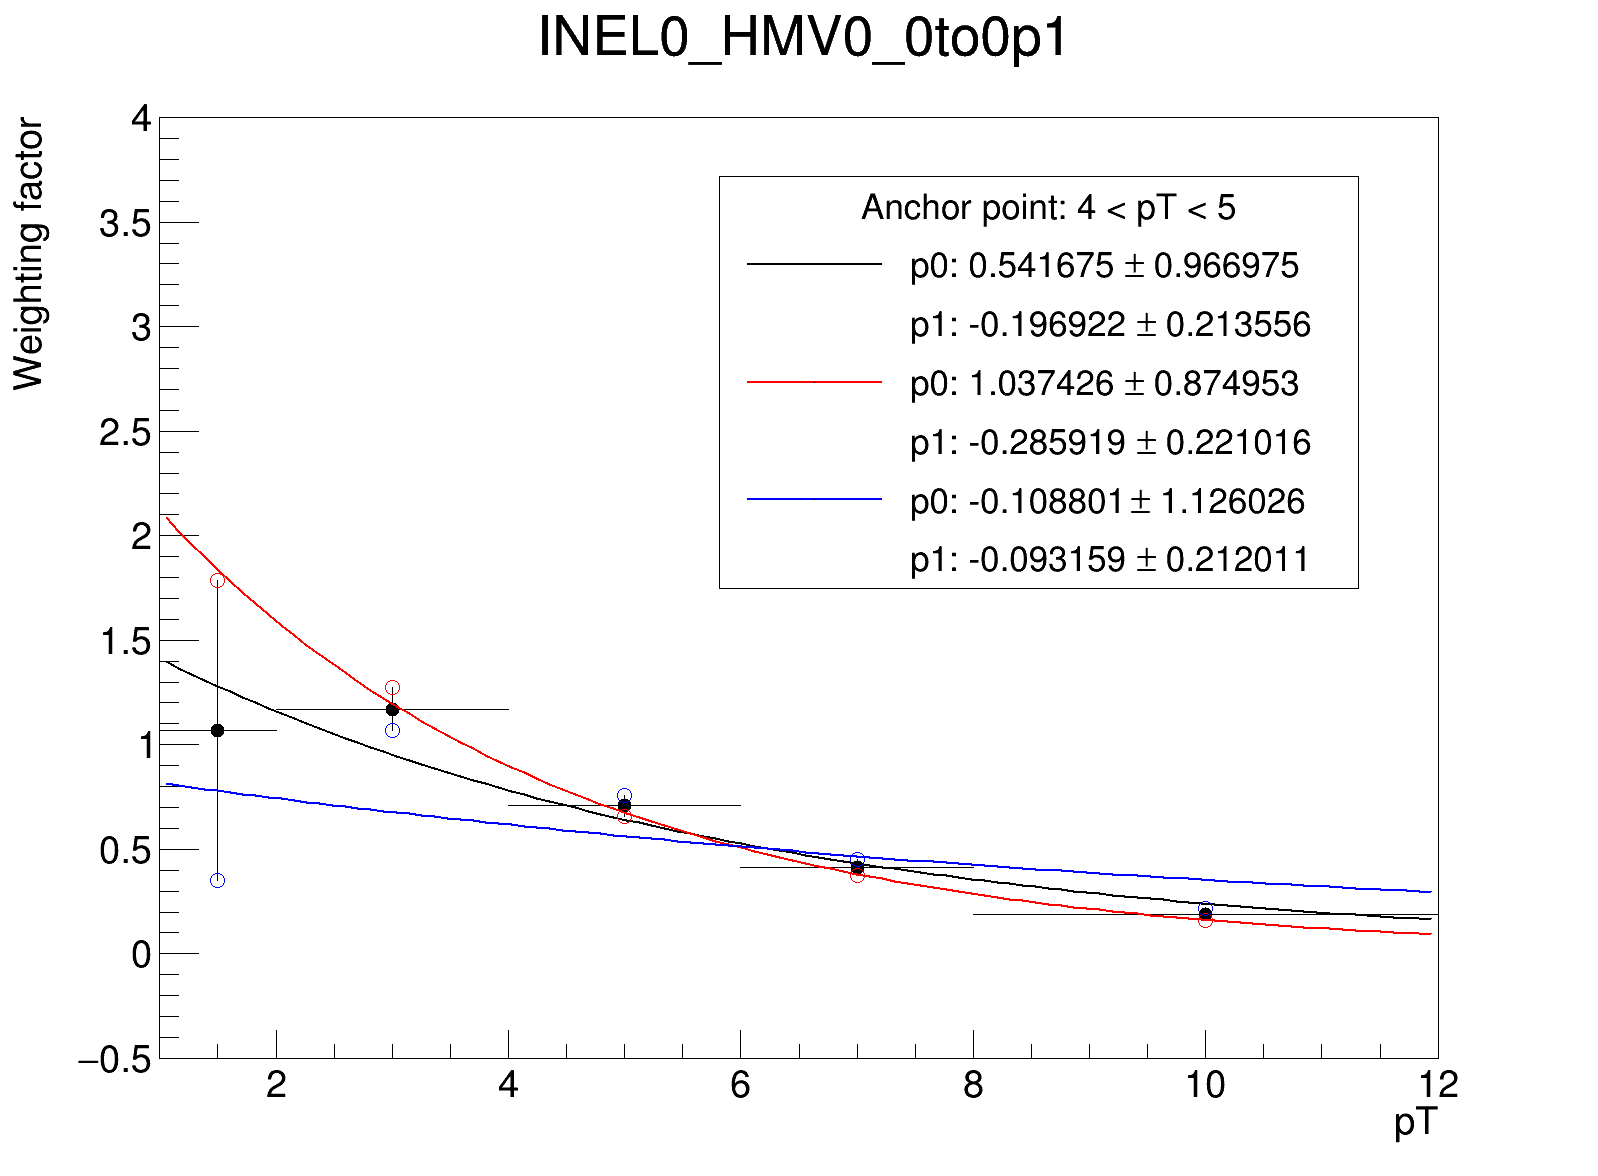
\includegraphics[width=0.45\textwidth]{plots/s2_pTW1to12_INEL0_HMV0_0to0p1.png}
    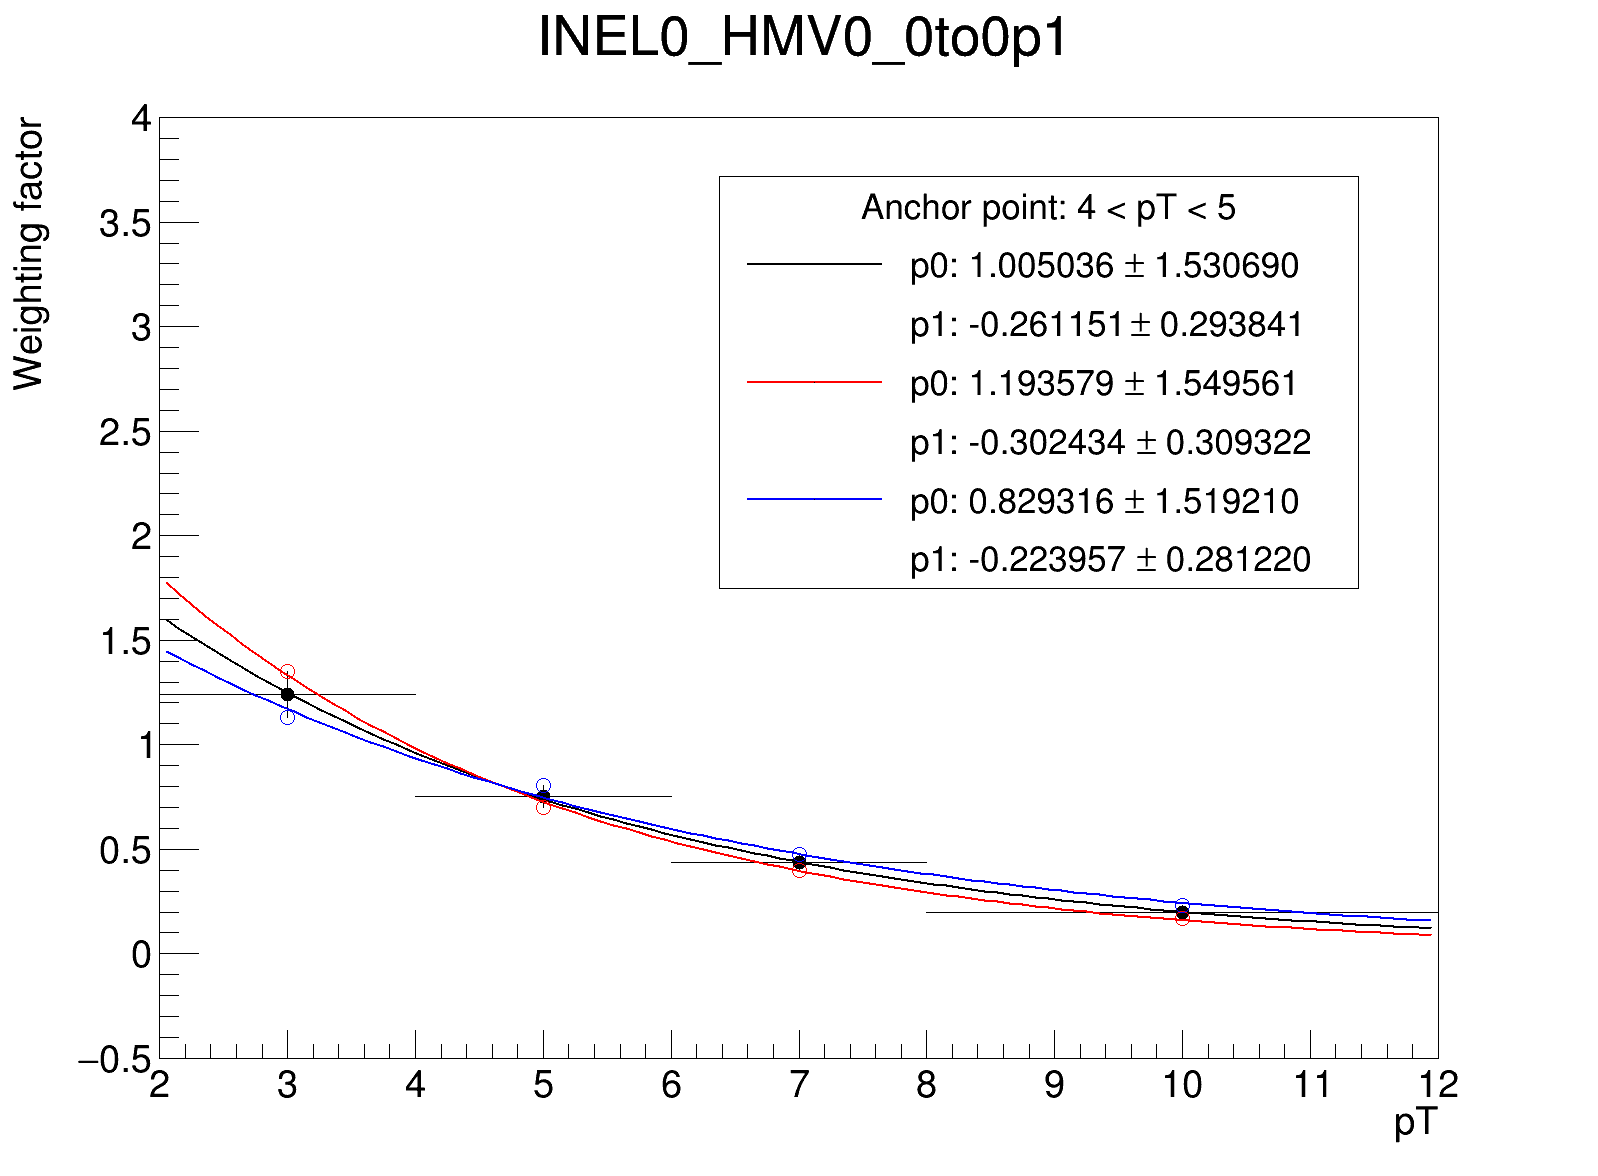
\includegraphics[width=0.45\textwidth]{plots/s2_pTW2to12_INEL0_HMV0_0to0p1.png}
    \caption{Study on weighting factor for each configuration: the points on each pad indicate data/MC ratio of normalized invariant cross-section (no weighting factors applied on MC at this stage) and the colored lines indicate weighting factors by fit (black: central, red/blue: variations with respect to the anchor point 4 $<$ \pt $<$ 5). Left column shows the factor obtained by including \pt range of 1 $<$ \pt $<$ 2 whie Right columne is not.}
    \label{fig:s2_pTW}
\end{figure}

\clearpage
%-----------------------------------------------
\subsubsection{Pair mass cut dependence on low \pt region}
\red{TBU}

\subsubsection{Multiplicity dependence of \Xib over-subtraction}
\red{TBU}